\newif\ifLaTeXe\LaTeXefalse
\expandafter\ifx\csname PackageError\endcsname\relax\LaTeXefalse
\else\LaTeXetrue\fi

\ifLaTeXe
  \documentclass{jarticle}
  \usepackage{SICE-SSI}
  \usepackage[dvips]{graphicx}
\else
  \documentstyle[SICE-SSI,epsbox]{jarticle}
\fi
\usepackage{comment}

\begin{document}

\title{手指使用量の常時計測のためのウェアラブルデバイスの開発}
\author{\ ○松本 崇斗 \ \ 矢野 史朗 \ \  近藤 敏之\ (東京農工大学)}

\abstract{
リハビリテーション介入の効果を定量的に評価するには,日常生活下の手指使用量を常時計測することが必要である.そこで本研究では,手指使用量を常時計測するためのウェアラブルデバイスの開発を行った.本デバイスは赤外線距離センサを用いて指の第二関節角度を推定する指輪型のデバイスである.角度推定の精度をカメラを用いて計測した関節角度と比較・評価した.評価指標にはMean Absolute Error$(MAE)$を用いた.3人の被験者がタスクを行った結果,$MAE$は$7.63^\circ \pm1.84^\circ(SD)$であった.結果より,本デバイスにより関節角度を推定可能であることが示唆された.
  }

\keyword{wearable device, finger monitoring, rehabilitaion}

\maketitle\thispagestyle{empty}
\pagestyle{empty}

\section{背景}
脳卒中麻痺リハビリテーションの目標は,食事,更衣,入浴などの日常生活動作ができるように患者の麻痺肢機能を改善することである.麻痺肢機能の改善を促進する介入方法の有効性を評価するためには,介入後の日常生活において,患者の麻痺肢使用量が実際に増えたか否かについて,リハビリテーションの効果を定量的に測る手法が必要である.しかしながら,病院やリハビリ施設で実施する検査では,質問紙やヒアリングによる調査が主体であり,日常生活における麻痺肢使用量を正確に評価することができない.\\
\ 例えば,片上肢麻痺患者の日常生活上での麻痺肢使用量を測る標準的手法としてMotor Activity Log(MAL)\cite{Taub2006},\cite{Uswatte2005}とAccelerometry\cite{Chen2005},\cite{Hayward2016}がある.MALは,医師が患者に対し,麻痺肢使用の量と質について直接問う,質問形式の手法であり,測定結果が患者の認知レベルによる影響や質問者の主観的影響を受ける問題がある.そのため,客観的な測定手法が必要である.また,Accelerometryは,加速度計が埋め込まれた腕時計型のウェアラブルデバイスで上肢の使用量を測る手法である.Accelerometryは麻痺肢の手首に装着することで,麻痺肢の使用量を測定する手法である.データ記録装置とバッテリーが内蔵されているため,麻痺肢使用量の常時計測に向いている\cite{VanDerPas2011}.しかし,この手法で計測される加速度データはノイズを多く含み,信頼性の高いデータを得ることができない.加速度データに混入するノイズは,測定された加速度が所定の時間内に,閾値を超える場合にのみ,麻痺肢使用のスコアを増加するといった手法の閾値フィルタを用いて低減することができる.このアプローチによって得られたスコアは日常生活において,腕を動かした時間と高い相関を持つことが示されている.しかし,閾値フィルタを使用したノイズ低減を行った場合,加速度が閾値に達しない小さな手の動きが見落とされる可能性がある.また,加速度計が手首に装着されているため,手首や手の精密な動きを計測できない問題がある.これらの理由から,Accelerometryは指の使用量の測定には向かない\cite{Uswatte2000}.

研究レベルではData gloveやGoniometer,Motion capture system\cite{Binh2014},\cite{Valtin2017}などが手首や手の使用量を測定するために使用される.しかしながら,これらの手法は指の動きの阻害,空間的な制限といった問題があるため,日常生活における長時間の常時計測には向いていない.さらに,磁力計と磁石の指輪を用いて手首や指の使用量を測定するManumeter\cite{Friedman2014}や,手の甲の皮膚の皺をパターン認識することによって,指ジェスチャを識別するBehind The Palm\cite{Recognition2017}といった手法が発表されているが,指の使用量の測定精度が低い,キャリブレーションによるユーザーへの負担が大きいと行った問題があり,依然として日常生活下の指の使用量を常時計測する手法は確立していない.本研究では,日常生活下の上肢片麻痺患者の麻痺肢使用,特に指の使用量を測る手法を提案し,手指使用量の常時測定のためのウェアラブルデバイスの開発を目的とする.


\section{方法}
\subsection{原理}
本研究の手指使用量の測定手法は,指の関節角度の変化が,指の使用量を反映するという仮定に基づく.関節角度の変化の推定には,ウェアラブルデバイスに搭載された赤外線距離センサを用いる.本デバイスは指の基節に装着して使用し,赤外線距離センサで,デバイスから中節までの距離を常時計測する.式(1)の関数を用い,測定された距離を指の関節角度に変換し,指の使用量を測る.距離を角度変換する模式図をFig.\ref{fig:principle}に示す.


\begin{figure}[h]
  \centering
  \includegraphics[width=0.8\linewidth]{fig/principle}
  \caption{Measurement principle}
  \label{fig:principle}
\end{figure}

\begin{equation}
\theta = \cos^{-1} \frac{x}{r}
\end{equation}

ここで,$r$は第二関節から指先までの長さ,$x$は最大屈曲時からの変化距離,$\theta$は最大伸展時からの変化角度である.

\subsection{ハードウェア}
本デバイスはLED(Osram SFH4550)とフォトトランジスタセンサ(Honeywell SD5410)で構成された赤外線距離センサを用いた指輪型のセンシング部と,手首に取り付けるデータ記録部から成るウェアラブルデバイスである.試作品をFig.\ref{fig:fal1}に示す.データ記録のため,マイコン基盤(Adafruit Faether M0)と32GBのSDcardを使用する.また,デバイスの電源として3.7V,900mAhのリポバッテリーを利用し,これにより24時間以上の連続電源供給が可能である.

\begin{figure}[h]
  \centering
  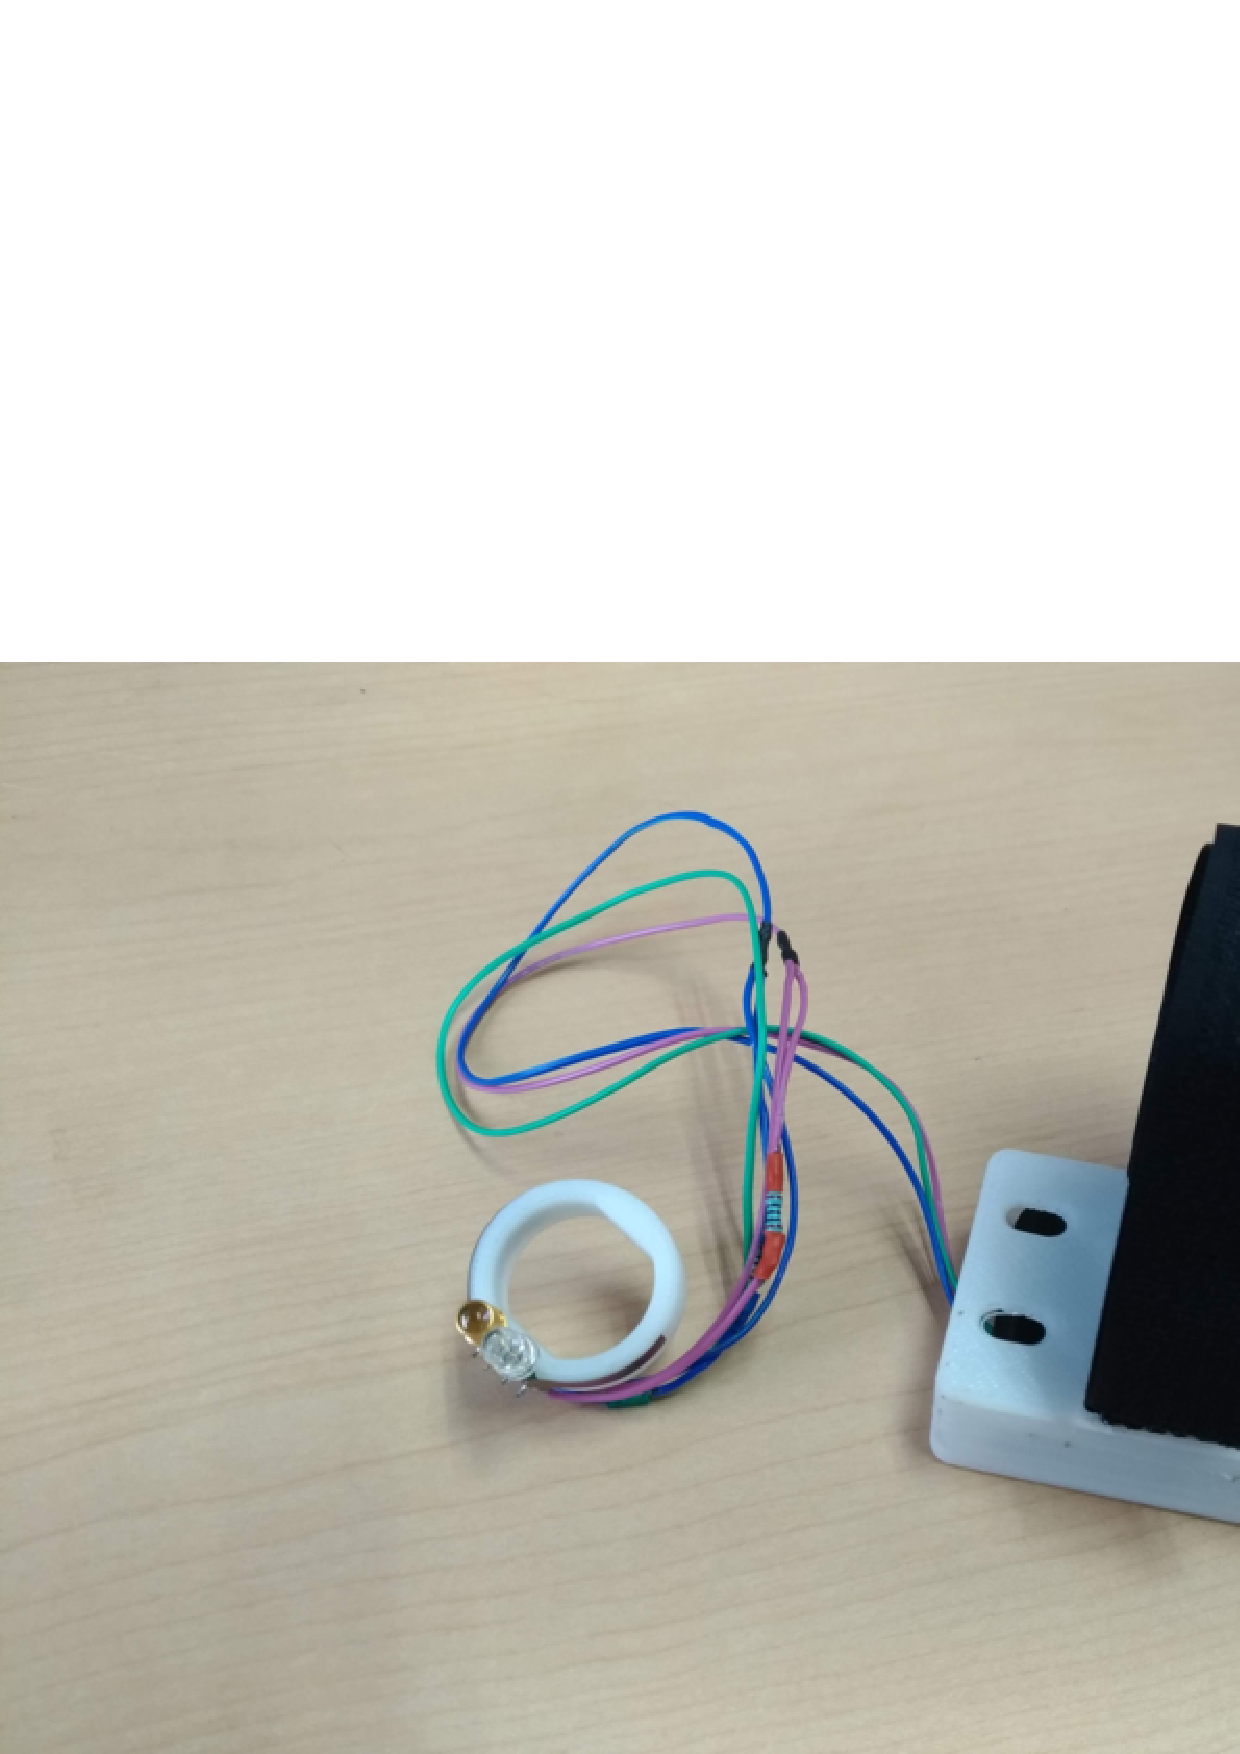
\includegraphics[width=0.8\linewidth]{fig/fal1}
  \caption{Hardware device}
  \label{fig:fal1}
\end{figure}

\begin{figure}[h]
  \centering
  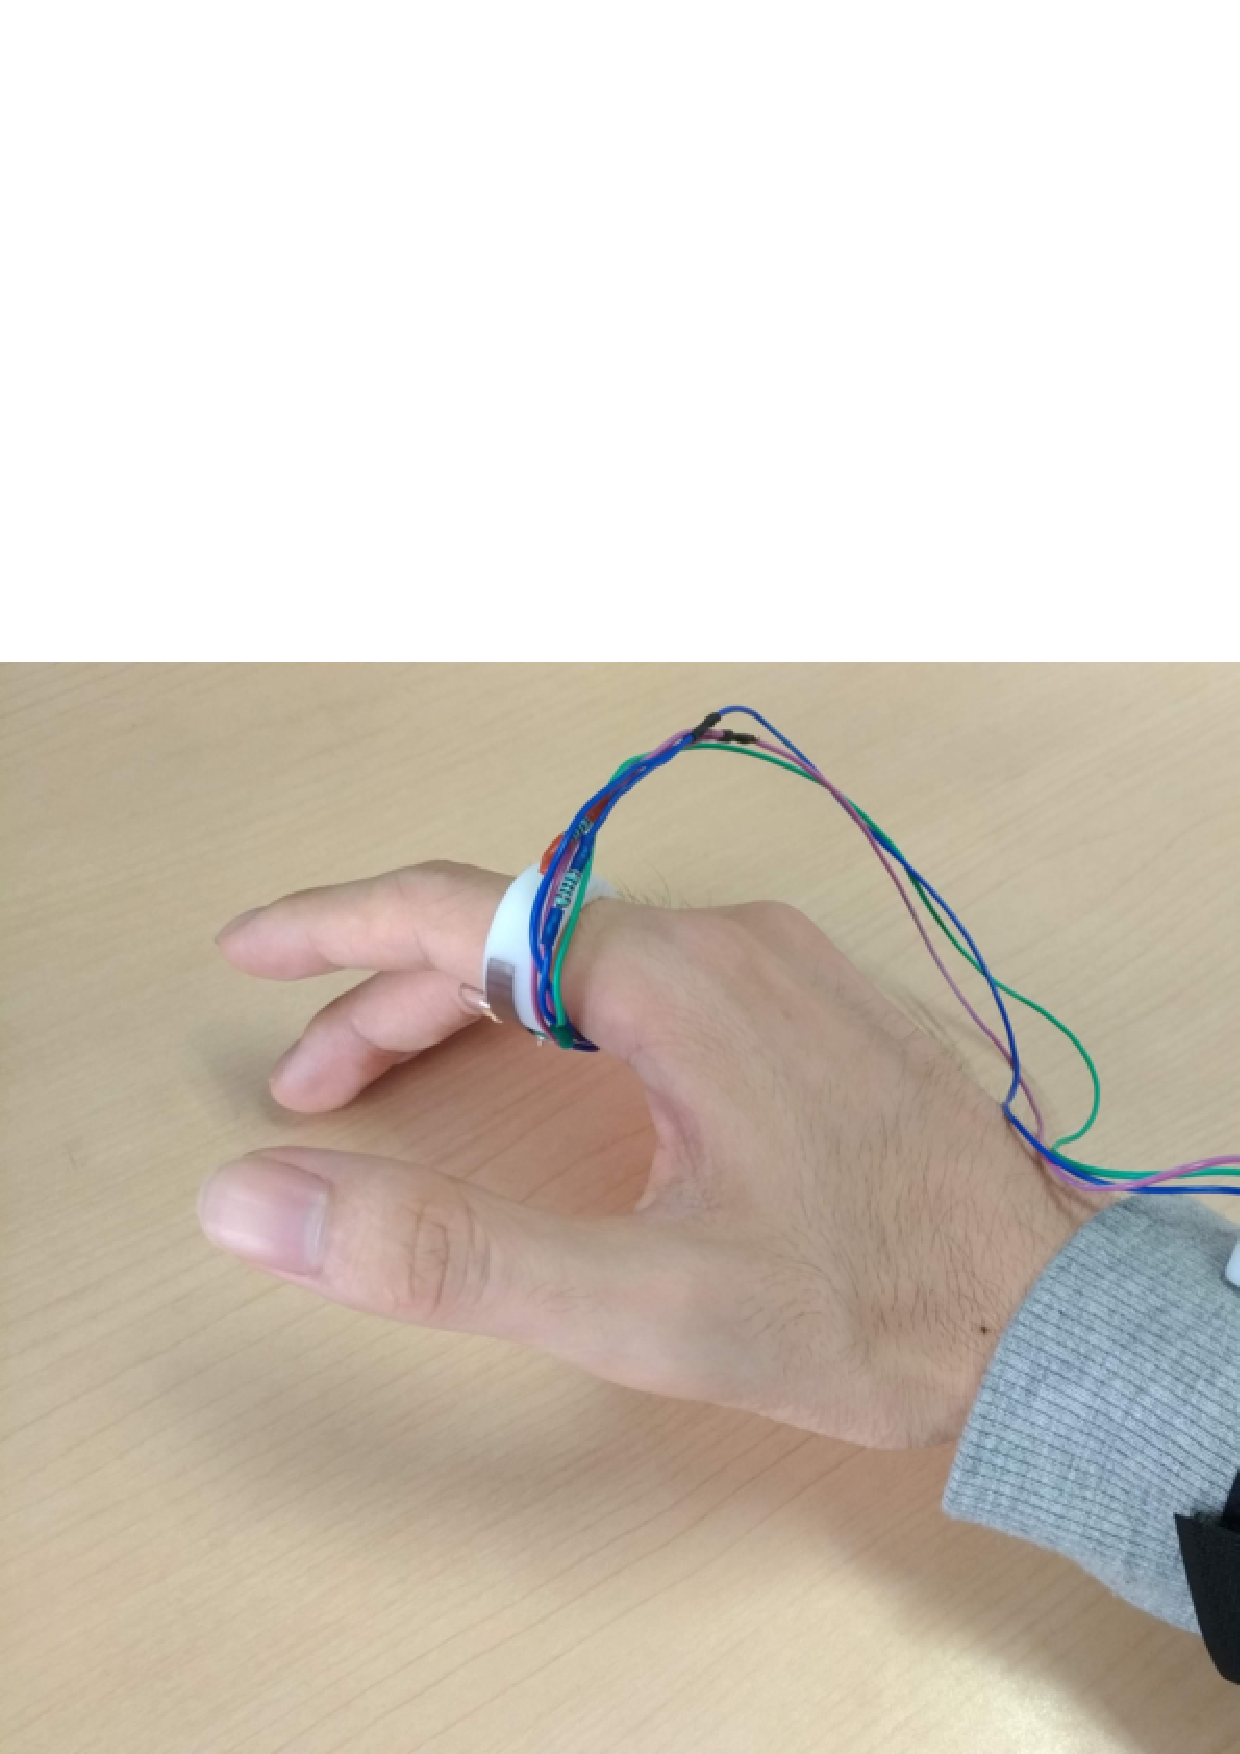
\includegraphics[width=0.8\linewidth]{fig/fal2}
  \caption{Ring worn on the index finger}
  \label{fig:gesture}
\end{figure}

本デバイスの指輪型の装着部分及び,バッテリーとマイコン基盤を収納するためのケースを3DCAD(Fusion 360)で設計し,3Dプリンタ(Dimension 1200es)で印刷し作成した.


\subsection{キャリブレーション}
赤外線距離センサは物体に反射し,フォトトランジスタで受光した赤外線の強度を計測することで,距離を推定する.
しかし,同じ距離であっても赤外線が反射する物体によっては,違う
受光量となる場合があり得る.これは物体によって光の反射率が違い,同じ距離で計測したとしても,フォトトランジスタで受け取る受光量が違ってくるためである.つまり,人によって,指の長さや皮膚の色が違うため,同じセンサ値であっても,本来の距離が変わる問題がある.この問題を解決するために,被験者ごとに皮膚の反射率を調べることが望ましいが,本システムは日常生活での使用を目的としており,キャリブレーション自体が簡単であることが求められる.
そのため,本システムでは計測される距離と受光量の関係を求め,簡単にキャリブレーションが可能な方法を提案する.キャリブレーションには以下の3つのパラメータを用いる.

\begin{itemize}
 \item デバイスを装着する指の長さ
 \item 指伸展時のセンサ情報
 \item 指屈曲時のセンサ情報
\end{itemize}


\section{実験および結果}
\subsection{ジェスチャ識別}
予備実験として健常者を対象に,本システムのジェスチャの認識精度を調査した.この実験の際は,LED(Osram SFH4550)とフォトトランジスタセンサ(Honeywell SD5410)の代わりに,赤外線距離センサ(Pololu QTR-1A)を2つ使用し,Fig.\ref{fig:sensor}の位置に取り付けた.

\begin{figure}[h]
  \centering
  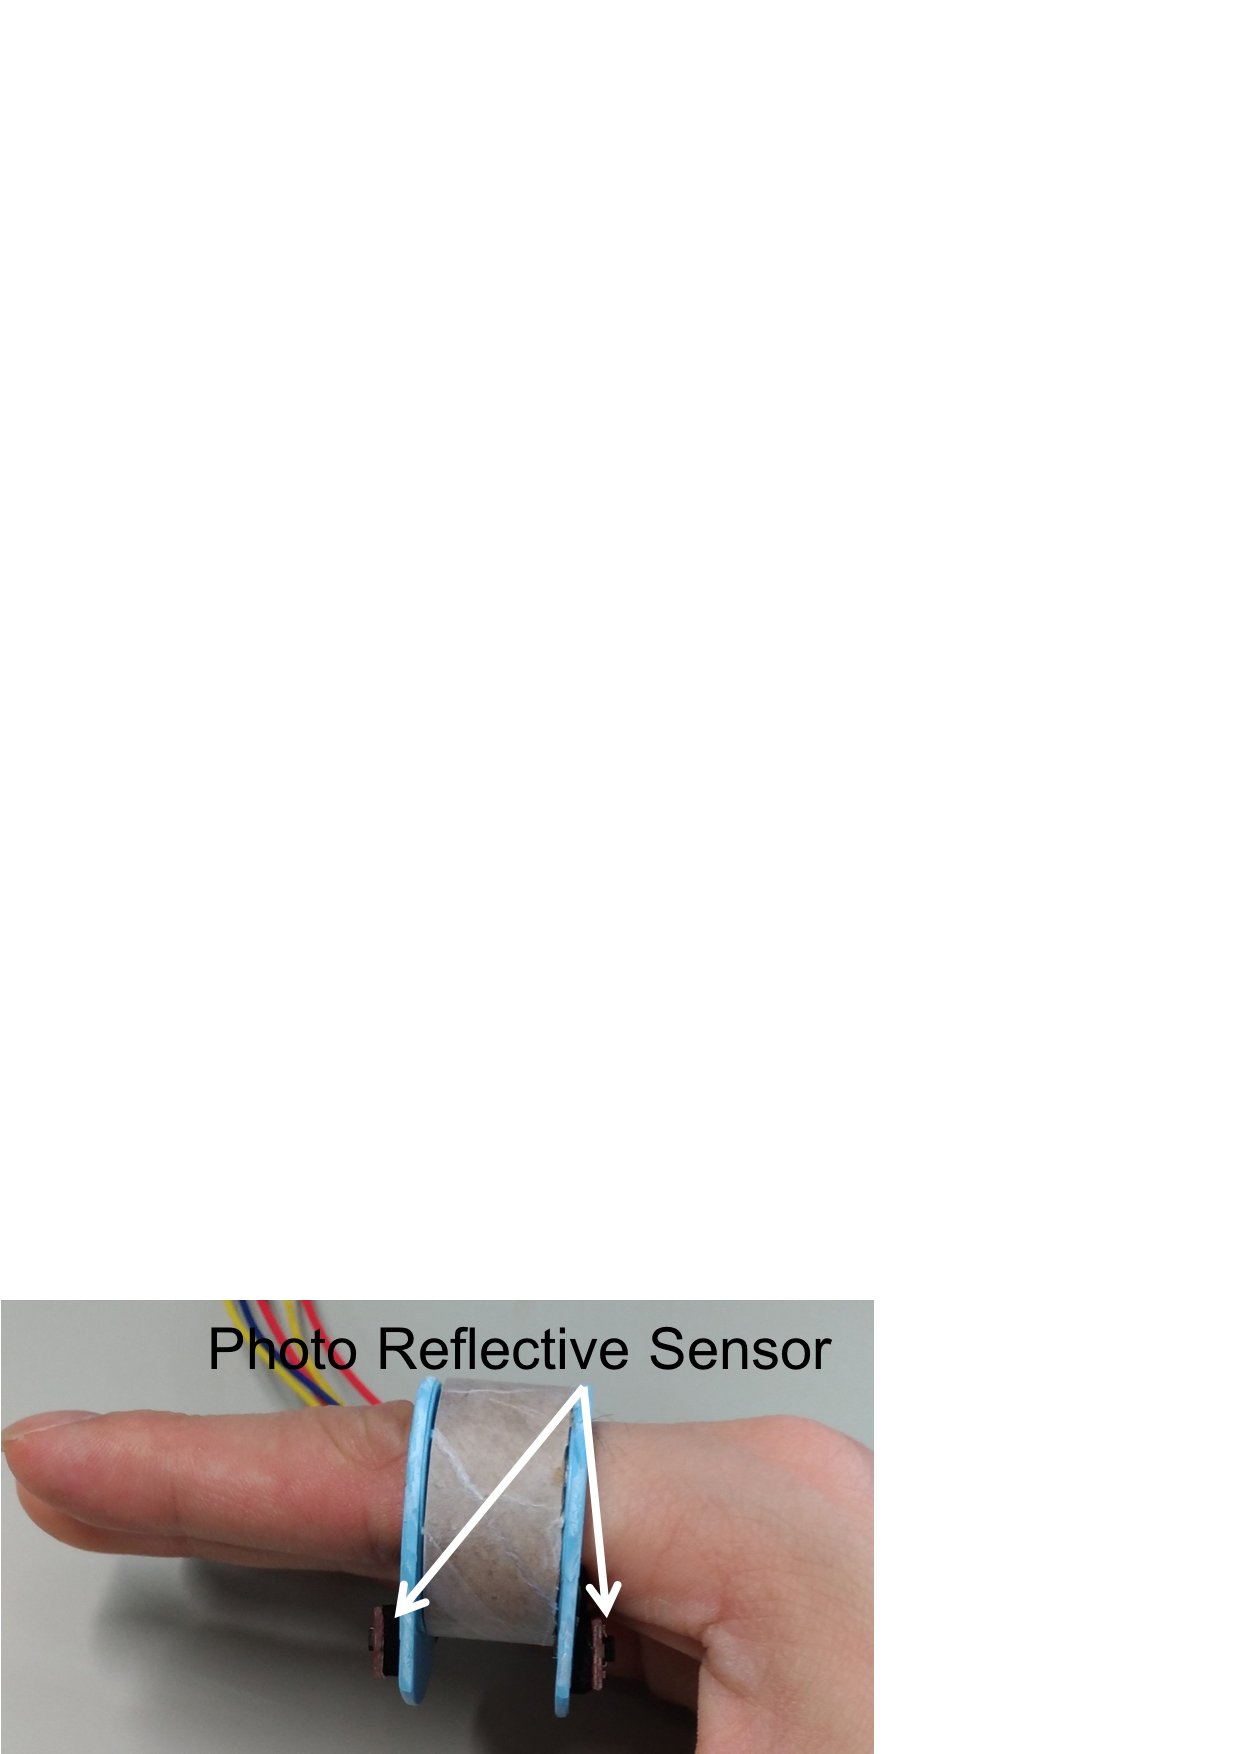
\includegraphics[width=0.8\linewidth]{fig/sensor}
  \caption{Mounting position of sensor}
  \label{fig:sensor}
\end{figure}

ジェスチャの種類をFig.\ref{fig:gesture}に示す.手指を閉じた状態(Fig.\ref{fig:gesture}の1),示指と母指で輪を作った状態(Fig.\ref{fig:gesture}の2),手指を開いた状態(Fig.\ref{fig:gesture}の3),計3つのジェスチャを指示し被験者に行ってもらった.被験者は椅子に座った状態で,本デバイスを装着した手でジェスチャを行った.一つのジェスチャを5秒間保持してもらい,その時のセンサーデータを収集した.5秒間のセンサーデータを時間で平均したセンサ値をジェスチャ識別のために利用した.
また,センサデータは各ジェスチャにつき60回記録し,五人の被験者センサデータを収集した.センシングの際のサンプルレートは100\ Hzとした.
合計で一人につき180データ(60データ$\times$3ジェスチャ)を収集した.


\begin{figure}[h]
  \centering
  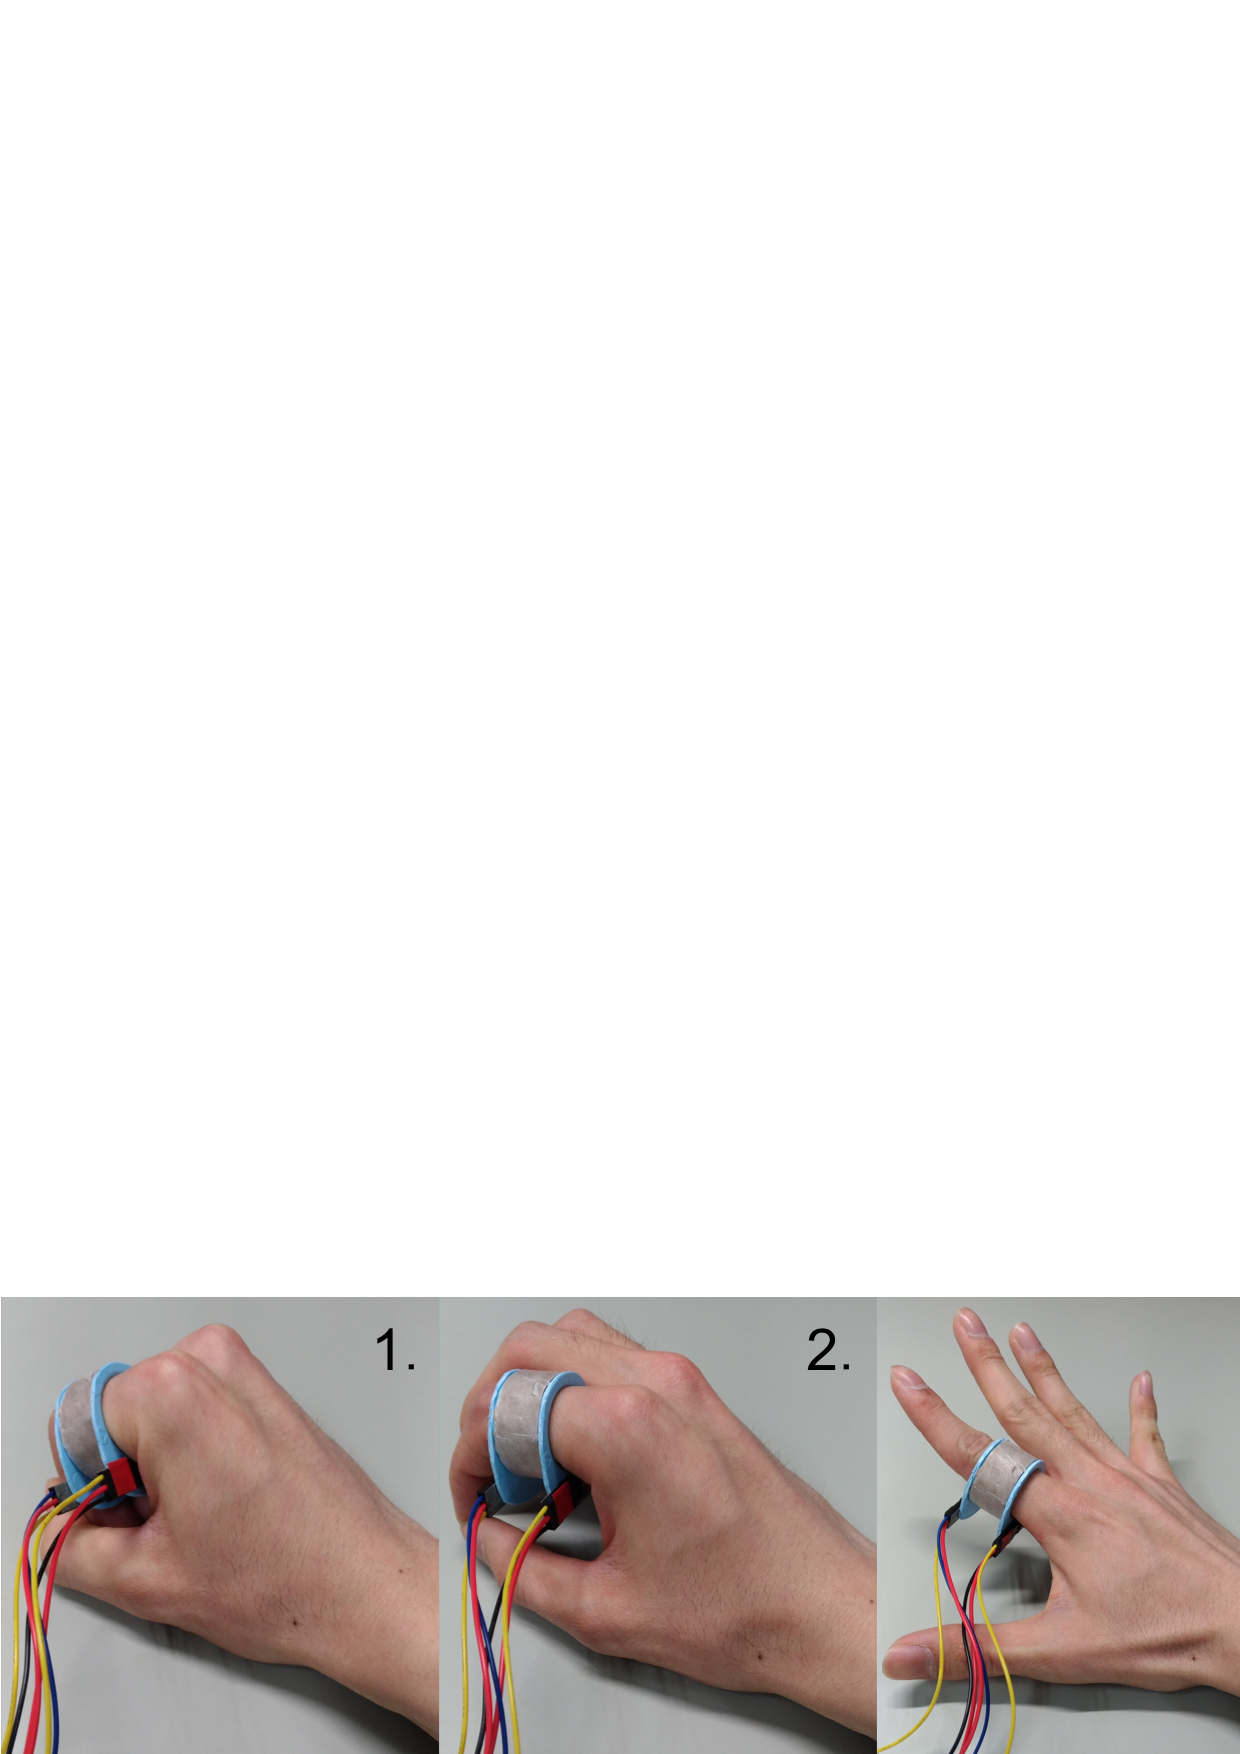
\includegraphics[width=0.8\linewidth]{fig/gesture}
  \caption{Prepared hand-gesture set}
  \label{fig:gesture}
\end{figure}

\begin{figure}[h]
  \centering
  \includegraphics[width=1.0\linewidth]{fig/confusion_matrix}
  \caption{Confusion matrix of 3-gesture}
  \label{fig:matrix}
\end{figure}

3つのジェスチャを識別するため,1対1分類法,線形Support Vector Machineを用いた.5人すべて,900データ(180データ$\times$5人)をジェスチャごとにラベル分けし,ジェスチャ識別に利用した.これらのデータの内,各ラベルに対し,データの80\%をトレーニングデータ,20\%をテストデータとした.

Fig.\ref{fig:matrix}より,ジェスチャ1と3を100\%の正解率で識別することが可能であることが分かった.5分割交差検証を行った結果,ジェスチャの平均正解率は98.9\%,分散3.9\%であった.この結果から本手法により3つのジェスチャの識別が可能であることが示された.

\subsection{関節角度推定}
本システムによって推定された第二関節角度の精度を調査した.以下の条件で実験を行なった.
被験者は第二指の中節に本デバイスとカラーマーカーを装着し,計測時間内に指の屈曲と伸展をそれぞれ3回ずつ行った.計測時間は20秒間で,センサのサンプルレートは10\ Hzとした.以上の条件のもと,3人の被験者が5セットタスクを行った.タスクを行う際,カメラで第二指を撮影し,関節角度の正解データとしてOpenCVのカラーマーカーを用いた関節角度の計測を行った.
また,精度の評価には式(2)のMean Absolute Error$(MAE)$を用いた.
\begin{equation}
MAE = \frac{1}{n} \sum^n_{k=1} |f_i-y_i|
\end{equation}
ここで$f_i$と$y_i$はそれぞれ時刻$i$のときの本システムによる推定関節角度とOpenCVによる関節角度の計測値である.
実験の結果,$MAE$は$7.63^\circ \pm1.84^\circ(SD)$であった.また,本システムによる推定関節角度とOpenCVによる関節角度の計測値の相関係数$R^2$は0.98であった.この結果から,本手法により,関節角度の推定が可能であることが示唆された.

\section{結論}
リハビリテーション介入の効果を定量的に測定する手法として,手指使用量の常時計測のためのウェアラブルデバイスの開発を行った.本デバイスは赤外線距離センサを用いて指の第二関節角度を推定する指輪型のデバイスである.結果より,本手法により関節角度を推定でき,手指使用量を計測可能であることが示唆された.

\section{謝辞}
本研究の一部は,JSPS KAKENHI (JP26120005,JP16H03219) の支援による.ここに謝意を表す.

\small
\bibliographystyle{jplain}
\bibliography{library}
\end{document}
